% !TeX program = xelatex
\documentclass[aspectratio=169,11pt]{beamer}

% -------------------------------------------------
% Packages
% -------------------------------------------------
\usepackage{kotex}
\usepackage{fontspec}
\usepackage{amsmath,amssymb,bm,mathtools}
\usepackage{booktabs,array}
\usepackage{xcolor}
\usepackage{colortbl}
\usepackage{tikz}
\usetikzlibrary{positioning,arrows.meta,calc,fit,decorations.pathreplacing}
\usepackage[most]{tcolorbox}
\usepackage{listings}
\usepackage{adjustbox}

% -------------------------------------------------
% Colors (same as the notes)
% -------------------------------------------------
\definecolor{deepblue}{RGB}{34,71,120}
\definecolor{softblue}{RGB}{239,246,253}
\definecolor{softgray}{RGB}{246,247,249}
\definecolor{softgreen}{RGB}{239,249,242}
\definecolor{softyellow}{RGB}{255,249,229}
\definecolor{codegray}{RGB}{248,248,248}

% -------------------------------------------------
% Beamer look
% -------------------------------------------------
\usetheme{default}
\usefonttheme[onlymath]{serif}
\setbeamertemplate{navigation symbols}{}
\setbeamersize{text margin left=8mm,text margin right=8mm}
\setbeamercolor{structure}{fg=deepblue}
\setbeamercolor{frametitle}{fg=deepblue}
\setbeamercolor{title}{fg=deepblue}
\setbeamerfont{frametitle}{size=\large,series=\bfseries}
\setbeamertemplate{itemize items}[circle]
\setbeamertemplate{enumerate items}[default]
\setbeamertemplate{frametitle}{%
  \vskip3mm
  {\usebeamerfont{frametitle}\usebeamercolor[fg]{frametitle}\insertframetitle\par}%
  \vskip1mm
  {\color{deepblue!45}\hrule height 0.6pt}%
  \vskip1mm}
\setbeamertemplate{footline}{%
  \hbox to\paperwidth{%
    \hspace*{8mm}{\color{black!45}\scriptsize NumPy로 만든 다층 신경망\ifx\insertsectionhead\empty\else\ \ $\cdot$\ \ \insertsectionhead\fi}%
    \hfill{\color{black!45}\scriptsize\insertframenumber\,/\,\inserttotalframenumber}\hspace*{8mm}}%
  \vskip2.5mm}
\setbeamertemplate{title page}{%
  \vfill
  \begin{center}
  {\color{deepblue}\Huge\bfseries\inserttitle\par}
  \vskip3mm
  {\color{deepblue!60}\rule{9cm}{0.8pt}\par}
  \vskip3mm
  {\large\insertsubtitle\par}
  \vskip8mm
  {\normalsize\insertdate\par}
  \end{center}
  \vfill}
\AtBeginSection[]{%
  \begin{frame}
  \vfill
  \centering
  {\color{deepblue!55}\Large\bfseries \insertsectionnumber\par}
  \vskip2mm
  {\color{deepblue}\LARGE\bfseries\insertsectionhead\par}
  \vskip3mm
  {\color{deepblue!50}\rule{7cm}{0.8pt}\par}
  \vfill
  \end{frame}}
\setlength{\leftmargini}{1.2em}
\setlength{\leftmarginii}{1.1em}

% -------------------------------------------------
% Boxes (same colors as the notes)
% -------------------------------------------------
\newtcolorbox{keybox}[1][]{colback=softblue,colframe=deepblue,boxrule=0.7pt,arc=2mm,
  title=#1,fonttitle=\bfseries\small,left=2mm,right=2mm,top=1mm,bottom=1mm,
  toptitle=0.5mm,bottomtitle=0.5mm}
\newtcolorbox{thinkbox}[1][]{colback=softyellow,colframe=orange!70!black,boxrule=0.6pt,arc=2mm,
  title=#1,fonttitle=\bfseries\small,left=2mm,right=2mm,top=1mm,bottom=1mm,
  toptitle=0.5mm,bottomtitle=0.5mm}
\newtcolorbox{remarkbox}[1][]{colback=softgray,colframe=black!45,boxrule=0.5pt,arc=2mm,
  title=#1,fonttitle=\bfseries\small,left=2mm,right=2mm,top=1mm,bottom=1mm,
  toptitle=0.5mm,bottomtitle=0.5mm}

% -------------------------------------------------
% Code style
% -------------------------------------------------
\lstdefinestyle{pythonstyle}{
  language=Python,
  backgroundcolor=\color{codegray},
  basicstyle=\ttfamily\scriptsize,
  keywordstyle=\bfseries\color{deepblue},
  commentstyle=\itshape\color{black!55},
  stringstyle=\color{black!75},
  numbers=none,
  frame=single,
  rulecolor=\color{black!25},
  breaklines=true,
  showstringspaces=false,
  tabsize=4,
  columns=fullflexible,
  keepspaces=true,
  aboveskip=1mm,
  belowskip=1mm
}
\lstset{style=pythonstyle}
% program output: no Python colors, light green background
\lstdefinestyle{outstyle}{style=pythonstyle,language={},backgroundcolor=\color{softgreen}}

% -------------------------------------------------
% Math commands (same as the notes)
% -------------------------------------------------
\newcommand{\R}{\mathbb{R}}
\newcommand{\vect}[1]{\bm{#1}}
\newcommand{\T}{^{\mathsf T}}
\newcommand{\pd}[2]{\frac{\partial #1}{\partial #2}}

\newcommand{\figcap}[1]{\par\vskip1mm{\centering\footnotesize\color{black!70}#1\par}}
\newcommand{\code}[1]{\texttt{#1}}

\graphicspath{{slides_figures/}}

\title{NumPy로 만든 다층 신경망}
\subtitle{\texttt{mnist\_mlp.py} 코드 읽기: 계층 $\cdot$ \texttt{MultiLayerNet} $\cdot$ 미니배치 학습 $\cdot$ 검증과 test}
\date{딥러닝개론및연습 $\cdot$ 2026년 2학기}

\begin{document}

% =================================================
\begin{frame}[plain]
\titlepage
\end{frame}

% =================================================
\begin{frame}{이번 시간의 핵심 질문}
\begin{keybox}[이번 시간의 핵심 질문]
\begin{itemize}
\item 실습에서 은닉층이 \textbf{하나}인 신경망을 계층 클래스로 만들었다 (\code{mnist\_lab.py})
\item 은닉층을 \textbf{여러 개} 쌓으려면 새 계층이나 새 역전파 식이 필요할까?
\item 여러 신경망 중 어느 것이 좋은지 \textbf{무엇으로} 비교해야 할까? test 데이터로 골라도 될까?
\item 학습이 끝난 신경망은 \textbf{어떤 숫자를} 헷갈릴까?
\end{itemize}
\end{keybox}
\vskip2mm
\begin{center}
\large $\Rightarrow$ \textbf{\code{mnist\_mlp.py}: NumPy만으로 만든 다층 신경망 (과제 2의 코드)}
\end{center}
\end{frame}

\begin{frame}{학습목표}
\begin{enumerate}
\item MNIST 데이터를 불러와 펼치기, 정규화, one-hot 인코딩, 훈련/검증 분할을 할 수 있다
\item \code{Affine}, \code{Relu}, \code{Sigmoid}, Softmax-손실 계층의 \code{forward}와 \code{backward}를 읽고 shape을 따라갈 수 있다
\item \code{MultiLayerNet}이 계층을 리스트에 쌓아 순전파와 역전파를 하는 방식을 설명할 수 있다
\item 미니배치 학습 함수 \code{train}의 epoch, iteration, 갱신을 설명할 수 있다
\item 설정을 \textbf{검증 정확도}로 고르고 test는 \textbf{한 번만} 평가하는 이유를 설명할 수 있다
\item 혼동행렬을 읽고 \code{experiments} 리스트를 고쳐 과제 2의 실험을 할 수 있다
\end{enumerate}
\end{frame}

\begin{frame}{목차}
\small
\tableofcontents
\end{frame}

% =================================================
\section{코드의 전체 구성}
% =================================================

\begin{frame}{\code{mnist\_mlp.py}의 여섯 부분}
\centering
\begin{adjustbox}{max width=\linewidth,max totalheight=0.62\textheight}
\begin{tikzpicture}[>=Latex,
  bk/.style={draw=deepblue,fill=softblue,rounded corners=3pt,align=center,font=\small,text width=36mm,minimum height=15mm}]
\node[bk] (s1) at (0,0)    {\textbf{1. 데이터}\\{\scriptsize 불러오기, 펼치기, 정규화, one-hot, 검증 분할}};
\node[bk] (s2) at (4.5,0)  {\textbf{2. 계층}\\{\scriptsize \code{Affine}, \code{Relu}, \code{Sigmoid}, Softmax-손실}};
\node[bk] (s3) at (9.0,0)  {\textbf{3. 신경망}\\{\scriptsize \code{class MultiLayerNet}}};
\node[bk] (s4) at (9.0,-2.6) {\textbf{4. 학습}\\{\scriptsize \code{train}: 미니배치 경사하강법}};
\node[bk] (s5) at (4.5,-2.6) {\textbf{5. 실험}\\{\scriptsize \code{experiments} 비교, 정확도 그래프}};
\node[bk] (s6) at (0,-2.6)   {\textbf{6. 최종 평가}\\{\scriptsize test 한 번, 혼동행렬}};
\draw[->,thick] (s1) -- (s2); \draw[->,thick] (s2) -- (s3); \draw[->,thick] (s3) -- (s4);
\draw[->,thick] (s4) -- (s5); \draw[->,thick] (s5) -- (s6);
\end{tikzpicture}
\end{adjustbox}
\vskip3mm
\raggedright
\begin{itemize}
\item 문제: MNIST $28\times28$ 손글씨 숫자 $\to$ $0$--$9$ 분류. \textbf{NumPy만} 쓴다 (그림은 matplotlib)
\item 계층 클래스(2)는 \code{mnist\_lab.py}와 주석만 빼면 \textbf{똑같다}. 새로 생긴 것은 3, 5, 6
\item 실행: 파일이 있는 폴더에서 \code{python mnist\_mlp.py} $\to$ \code{figures} 폴더에 그림 2개 저장
\end{itemize}
\end{frame}

\begin{frame}{\code{mnist\_lab.py}와 무엇이 다른가}
\centering
\small
\renewcommand{\arraystretch}{1.3}
\begin{tabular}{>{\raggedright}p{3.0cm}>{\raggedright}p{4.8cm}>{\raggedright\arraybackslash}p{5.0cm}}
\toprule
& \textbf{\code{mnist\_lab.py} (실습)} & \textbf{\code{mnist\_mlp.py} (이번 시간)} \\
\midrule
신경망 & \code{TwoLayerNet}: 은닉층 1개 & \code{MultiLayerNet}: 은닉층 \textbf{몇 개든} \\
계층 클래스 & \code{Affine}, \code{Relu}, \ldots & \textbf{같음} \\
데이터 & 훈련 60000 / test 10000 & 훈련 55000 / \textbf{검증 5000} / test 10000 \\
실험 & 설정 하나 & 여러 설정을 \textbf{검증 정확도로 비교} \\
결과 확인 & 손실 그래프, 예측 이미지 & 정확도 비교 그래프, \textbf{혼동행렬} \\
\bottomrule
\end{tabular}
\vskip3mm
\raggedright
\begin{itemize}
\item 층을 깊게 쌓는 데 필요한 것은 \textbf{새 수식이 아니라 반복문}이다
\end{itemize}
\end{frame}

% =================================================
\section{데이터 준비}
% =================================================

\begin{frame}[fragile]{1. 데이터 불러오기: \code{load\_mnist}}
\begin{lstlisting}
def load_mnist():
    """Return (x_train, t_train), (x_test, t_test): images (N,28,28), labels (N,)."""
    try:
        from tensorflow.keras.datasets import mnist   # if TensorFlow is installed
        return mnist.load_data()
    except ImportError:
        from sklearn.datasets import fetch_openml     # otherwise download from OpenML
        X, y = fetch_openml("mnist_784", version=1, as_frame=False, return_X_y=True)
        X = X.reshape(-1, 28, 28).astype(np.uint8)
        y = y.astype(np.int64)
        return (X[:60000], y[:60000]), (X[60000:], y[60000:])

(x_all_o, t_all_o), (x_test_o, t_test_o) = load_mnist()
\end{lstlisting}
\begin{itemize}
\item \code{try}/\code{except}: TensorFlow가 있으면 그것으로, \textbf{없으면} scikit-learn으로 내려받는다
\item 어느 쪽이든 결과는 같다: 이미지 \code{(N, 28, 28)}, 픽셀 $0$--$255$, 정답 \code{(N,)} (클래스 번호)
\item 앞 $60000$장이 훈련용, 뒤 $10000$장이 test용. 이름 끝의 \code{\_o}는 \textbf{원본}(original)
\end{itemize}
\end{frame}

\begin{frame}[fragile]{1. 펼치기, 정규화, one-hot}
\begin{lstlisting}
x_all  = x_all_o.reshape(x_all_o.shape[0], -1) / 255.0      # (60000, 784)
x_test = x_test_o.reshape(x_test_o.shape[0], -1) / 255.0    # (10000, 784)
t_all  = np.eye(10)[t_all_o]                                 # (60000, 10)
t_test = np.eye(10)[t_test_o]                                # (10000, 10)
\end{lstlisting}
\begin{columns}[T,onlytextwidth]
\begin{column}{0.52\textwidth}
\small
\begin{itemize}
\item \code{reshape(N, -1)}: 이미지 한 장 $28\times28$ $\to$ 행벡터 하나 ($784$). \code{-1}은 ``나머지를 알아서''
\item \code{/ 255.0}: 픽셀 값을 $0$--$1$로
\item \code{np.eye(10)}: $10\times10$ 단위행렬. 그 \textbf{$k$번째 행}이 바로 $k$의 one-hot 벡터
\item \code{np.eye(10)[t]}: 행을 정답 번호로 골라 한꺼번에 one-hot
\end{itemize}
\end{column}
\begin{column}{0.44\textwidth}
\begin{lstlisting}
labels = np.array([5, 0, 4])
print(np.eye(10)[labels].astype(int))
\end{lstlisting}
\begin{lstlisting}[style=outstyle]
[[0 0 0 0 0 1 0 0 0 0]
 [1 0 0 0 0 0 0 0 0 0]
 [0 0 0 0 1 0 0 0 0 0]]
\end{lstlisting}
\end{column}
\end{columns}
\end{frame}

\begin{frame}[fragile]{1. 훈련 / 검증 분할}
\begin{lstlisting}
perm = np.random.permutation(x_all.shape[0])
val_idx, train_idx = perm[:5000], perm[5000:]
x_train, t_train = x_all[train_idx], t_all[train_idx]       # (55000, 784)
x_val,   t_val   = x_all[val_idx],   t_all[val_idx]         # (5000, 784)
\end{lstlisting}
\begin{lstlisting}[style=outstyle]
train: (55000, 784)  validation: (5000, 784)  test: (10000, 784)
\end{lstlisting}
\centering
\footnotesize
\renewcommand{\arraystretch}{1.15}
\begin{tabular}{lrl}
\toprule
\textbf{데이터} & \textbf{개수} & \textbf{용도} \\
\midrule
훈련 (train) & 55000 & 매개변수 $W$, $B$를 학습 \\
검증 (validation) & 5000 & 여러 \textbf{설정}(층 수, 넓이, 학습률, \ldots) 중 하나를 고르기 \\
테스트 (test) & 10000 & 고른 신경망의 최종 성능. \textbf{마지막에 한 번만} \\
\bottomrule
\end{tabular}
\raggedright
\small
\begin{itemize}
\item \code{permutation}: $0,\ldots,59999$를 무작위로 섞은 배열. 앞 $5000$개 번호를 검증용으로 뗀다
\end{itemize}
\end{frame}

\begin{frame}{왜 검증 데이터가 따로 필요한가}
\begin{itemize}
\item 설정을 고를 때 test 정확도를 보면 $\to$ \textbf{test 데이터에 맞춰} 설정을 고른 셈이 된다
\item 그러면 test 정확도는 ``처음 보는 데이터''에 대한 성능이 아니게 되고, 실제보다 \textbf{좋게} 나온다
\end{itemize}
\vskip2mm
\begin{keybox}[세 데이터의 역할]
\begin{enumerate}
\item \textbf{훈련 데이터}로 매개변수를 학습한다
\item \textbf{검증 데이터}로 여러 설정을 비교해 가장 좋은 것을 고른다
\item 고른 신경망을 \textbf{test 데이터}로 \textbf{단 한 번} 평가해 보고한다
\end{enumerate}
\end{keybox}
\begin{thinkbox}[비유]
\small
검증 데이터는 \textbf{모의고사}, test 데이터는 \textbf{수능}. 모의고사 점수로 공부 방법을 바꾸는 것은 괜찮지만,
수능 문제를 미리 보고 공부하면 수능 점수는 실력을 나타내지 못한다.
\end{thinkbox}
\end{frame}

% =================================================
\section{계층 클래스}
% =================================================

\begin{frame}{계층의 공통 규칙}
\centering
\begin{adjustbox}{max width=\linewidth}
\begin{tikzpicture}[>=Latex,
  ly/.style={draw=deepblue,fill=softblue,rounded corners=2pt,minimum width=20mm,minimum height=11mm,font=\small,align=center}]
\node[ly] (L) at (0,0) {계층\\{\scriptsize (입력을 기억)}};
\draw[->,thick] (-3.2,0.3) -- node[above,font=\small]{입력 $X$} (-1.0,0.3);
\draw[->,thick] (1.0,0.3) -- node[above,font=\small]{출력} (3.2,0.3);
\draw[<-,thick,red!75!black,dashed] (-3.2,-0.3) -- node[below,font=\small]{$\partial L/\partial(\text{입력})$} (-1.0,-0.3);
\draw[<-,thick,red!75!black,dashed] (1.0,-0.3) -- node[below,font=\small]{$\partial L/\partial(\text{출력})$} (3.2,-0.3);
\node[font=\small,anchor=west] at (3.5,0.3) {\code{forward}};
\node[font=\small,anchor=west,red!75!black] at (3.5,-0.3) {\code{backward}};
\end{tikzpicture}
\end{adjustbox}
\vskip3mm
\raggedright
\begin{itemize}
\item \code{forward(입력)}: 출력을 계산하고, 역전파에 필요한 값을 \code{self}에 \textbf{저장}한다
\item \code{backward(출력에 대한 기울기)}: 저장한 값으로 \textbf{입력에 대한 기울기}를 돌려준다 (연쇄법칙)
\item 매개변수가 있는 계층(\code{Affine})은 \code{backward}에서 \code{self.dW}, \code{self.dB}도 저장한다
\item 그래서 계층을 \textbf{몇 개를 이어 붙이든} 앞에서부터 \code{forward}, 뒤에서부터 \code{backward}만 부르면 된다
\end{itemize}
\vskip1mm
\begin{remarkbox}
\small 기호: 미니배치 크기 $h$, 입력 $X\in\R^{h\times l}$, 가중치 $W\in\R^{l\times m}$, 점수 $U$, 정답(one-hot) $T$, softmax 출력 $Y$
\end{remarkbox}
\end{frame}

\begin{frame}[fragile]{2. \code{Affine} 계층: $A=XW+B$}
\begin{columns}[T,onlytextwidth]
\begin{column}{0.55\textwidth}
\begin{lstlisting}
class Affine:
    def __init__(self, W, B):
        self.W = W          # (l, m)
        self.B = B          # (1, m)
        self.X = None
        self.dW = None
        self.dB = None

    def forward(self, X):
        self.X = X
        return X @ self.W + self.B

    def backward(self, dA):
        self.dW = self.X.T @ dA
        self.dB = np.sum(dA, axis=0, keepdims=True)
        return dA @ self.W.T
\end{lstlisting}
\end{column}
\begin{column}{0.42\textwidth}
\small
\[
\pd{L}{W}=X\T\pd{L}{A},\quad
\pd{L}{B}=\sum_{\text{행}}\pd{L}{A}
\]
\[
\pd{L}{X}=\pd{L}{A}\,W\T
\]
\renewcommand{\arraystretch}{1.1}
\scriptsize
\setlength{\tabcolsep}{3pt}
\noindent\begin{adjustbox}{max width=0.95\linewidth}
\begin{tabular}{ll}
\toprule
\textbf{식} & \textbf{shape} \\
\midrule
\code{X @ W + B} & $(h,l)(l,m)+(1,m)\to(h,m)$ \\
\code{X.T @ dA} & $(l,h)(h,m)\to(l,m)$ \\
\code{sum(dA,axis=0)} & $(h,m)\to(1,m)$ \\
\code{dA @ W.T} & $(h,m)(m,l)\to(h,l)$ \\
\bottomrule
\end{tabular}
\end{adjustbox}
\end{column}
\end{columns}
\small
\begin{itemize}
\item 기울기의 shape은 \textbf{그 변수의 shape과 같다}: \code{dW}는 \code{W}와, \code{dX}는 \code{X}와
\item \code{+ self.B}: $(1,m)$이 $h$개의 행에 \textbf{브로드캐스팅} $\to$ 역전파에서는 행끼리 \textbf{더한다}
\end{itemize}
\end{frame}

\begin{frame}[fragile]{2. 활성화 계층: \code{Relu}, \code{Sigmoid}}
\begin{columns}[T,onlytextwidth]
\begin{column}{0.48\textwidth}
\begin{lstlisting}
class Relu:
    def __init__(self):
        self.mask = None

    def forward(self, A):
        self.mask = (A > 0)
        return np.where(self.mask, A, 0.0)

    def backward(self, dZ):
        return np.where(self.mask, dZ, 0.0)
\end{lstlisting}
\small
\begin{itemize}
\item \code{mask}: 입력이 양수였던 자리 (\code{True}/\code{False})
\item 역전파: 양수였던 자리만 기울기를 \textbf{그대로} 통과, 나머지는 $0$
\end{itemize}
\end{column}
\begin{column}{0.48\textwidth}
\begin{lstlisting}
class Sigmoid:
    def __init__(self):
        self.Z = None

    def forward(self, A):
        self.Z = 1.0 / (1.0 + np.exp(-A))
        return self.Z

    def backward(self, dZ):
        return dZ * self.Z * (1.0 - self.Z)
\end{lstlisting}
\small
\begin{itemize}
\item $\sigma'(a)=\sigma(a)\bigl(1-\sigma(a)\bigr)$이므로 \textbf{출력} $Z$만 저장하면 된다
\item 모두 \textbf{원소별} 연산: shape이 바뀌지 않는다
\end{itemize}
\end{column}
\end{columns}
\end{frame}

\begin{frame}[fragile]{2. softmax: 최댓값을 빼는 이유}
\begin{columns}[T,onlytextwidth]
\begin{column}{0.50\textwidth}
\begin{lstlisting}
def softmax(U):
    U = U - np.max(U, axis=1, keepdims=True)
    expU = np.exp(U)
    return expU / np.sum(expU, axis=1, keepdims=True)
\end{lstlisting}
\begin{lstlisting}
U = np.array([[1000.0, 1001.0, 1002.0]])
naive = np.exp(U) / np.sum(np.exp(U), axis=1, keepdims=True)
print("naive softmax:", naive)
print("softmax      :", np.round(softmax(U), 4))
\end{lstlisting}
\begin{lstlisting}[style=outstyle]
naive softmax: [[nan nan nan]]
softmax      : [[0.09   0.2447 0.6652]]
\end{lstlisting}
\end{column}
\begin{column}{0.46\textwidth}
\small
\begin{itemize}
\item $e^{1000}$은 컴퓨터가 나타낼 수 없다 (\code{inf}) $\to$ $\infty/\infty=$ \code{nan}
\item 모든 점수에서 같은 수 $c$를 빼도 softmax는 같다:
\[
\frac{e^{u_k-c}}{\sum_j e^{u_j-c}}=\frac{e^{u_k}}{\sum_j e^{u_j}}
\]
\item 행마다 최댓값을 빼면 가장 큰 지수가 $e^0=1$ $\to$ 넘침이 없다
\item \code{axis=1}: 데이터 하나(\textbf{행})마다
\end{itemize}
\end{column}
\end{columns}
\end{frame}

\begin{frame}[fragile]{2. 출력층: \code{SoftmaxWithCrossEntropy}}
\begin{columns}[T,onlytextwidth]
\begin{column}{0.53\textwidth}
\begin{lstlisting}[basicstyle=\ttfamily\fontsize{7.5}{8.4}\selectfont]
class SoftmaxWithCrossEntropy:
    def __init__(self):
        self.Y = None
        self.T = None

    def forward(self, U, T):
        self.T = T
        self.Y = softmax(U)
        h = U.shape[0]
        return -np.sum(T * np.log(self.Y + 1e-12)) / h

    def backward(self):
        h = self.T.shape[0]
        return (self.Y - self.T) / h
\end{lstlisting}
\end{column}
\begin{column}{0.44\textwidth}
\small
\[
L=-\frac1h\sum_{n=1}^{h}\sum_{k=1}^{10}t_{nk}\log y_{nk}
\]
\[
\pd{L}{U}=\frac{1}{h}\,(Y-T)
\]
\begin{itemize}
\item \code{1e-12}: $\log 0=-\infty$를 피한다
\item 손실은 미니배치의 \textbf{평균}. 그래서 $h$로 나눈다
\item 역전파의 출발점이 \textbf{예측 $-$ 정답}
\end{itemize}
\end{column}
\end{columns}
\begin{keybox}
\small
$h$로 나누는 곳은 \textbf{여기 한 곳뿐}이다. 앞 계층들은 이 $\frac1h$이 곱해진 기울기를 받아서 그대로 전달하므로,
\code{Affine}의 \code{dW}, \code{dB}도 자동으로 미니배치 평균의 기울기가 된다.
\end{keybox}
\end{frame}

\begin{frame}[fragile]{2. 비교용: \code{SoftmaxWithSquaredError}}
\begin{lstlisting}
class SoftmaxWithSquaredError:
    def forward(self, U, T):
        self.T = T
        self.Y = softmax(U)
        h = U.shape[0]
        return 0.5 * np.sum((self.Y - self.T) ** 2) / h

    def backward(self):
        h = self.T.shape[0]
        R = self.Y - self.T
        return self.Y * (R - np.sum(self.Y * R, axis=1, keepdims=True)) / h
\end{lstlisting}
\begin{itemize}
\item softmax 출력에 \textbf{제곱 오차}를 쓴 손실 (\code{\_\_init\_\_}은 위와 같아서 생략)
\item 역전파 식이 $\frac1h(Y-T)$처럼 간단하지 않다: softmax의 미분이 그대로 남는다
\item 과제 2에서 \code{loss="se"}로 바꾸면 이 계층을 쓴다. cross entropy와 학습 속도를 비교해 보자
\end{itemize}
\end{frame}

% =================================================
\section{\texttt{MultiLayerNet}: 계층 쌓기}
% =================================================

\begin{frame}{구조: Affine과 활성화를 번갈아 쌓는다}
\centering
\begin{adjustbox}{max width=\linewidth}
\begin{tikzpicture}[>=Latex,
  lay/.style={draw=deepblue,fill=softblue,rounded corners=2pt,minimum width=14mm,minimum height=20mm,font=\small},
  act/.style={draw=black!55,fill=softgray,rounded corners=2pt,minimum width=11mm,minimum height=20mm,font=\small}]
\node[font=\small,align=center] (x) at (-1.1,0) {$X$\\{\scriptsize $(h,784)$}};
\node[lay] (a1) at (0.6,0) {Affine};
\node[act] (r1) at (2.1,0) {ReLU};
\node[lay] (a2) at (3.6,0) {Affine};
\node[act] (r2) at (5.1,0) {ReLU};
\node[lay] (a3) at (6.6,0) {Affine};
\node[draw,rounded corners=2pt,minimum width=16mm,minimum height=20mm,font=\small,fill=orange!12,align=center] (sm) at (8.5,0) {Softmax\\--CE};
\node[font=\small] (L) at (10.0,0) {$L$};
\draw[->] (x) -- (a1); \draw[->] (a1) -- (r1); \draw[->] (r1) -- (a2); \draw[->] (a2) -- (r2);
\draw[->] (r2) -- (a3); \draw[->] (a3) -- node[above,font=\scriptsize]{$U$} (sm); \draw[->] (sm) -- (L);
\node[font=\scriptsize] at (1.35,1.35) {$784\to100$};
\node[font=\scriptsize] at (4.35,1.35) {$100\to100$};
\node[font=\scriptsize] at (6.6,1.35) {$100\to10$};
\draw[decorate,decoration={brace,amplitude=5pt,mirror}] (-0.1,-1.2) -- (2.65,-1.2)
  node[midway,below=6pt,font=\small] {은닉층 1};
\draw[decorate,decoration={brace,amplitude=5pt,mirror}] (2.9,-1.2) -- (5.65,-1.2)
  node[midway,below=6pt,font=\small] {은닉층 2};
\draw[decorate,decoration={brace,amplitude=5pt,mirror}] (5.9,-1.2) -- (9.3,-1.2)
  node[midway,below=6pt,font=\small] {출력층};
\node[font=\scriptsize,black!60,anchor=west] at (-0.1,-2.25) {\code{self.layers} (리스트)};
\node[font=\scriptsize,black!60] at (8.5,-2.25) {\code{self.last}};
\end{tikzpicture}
\end{adjustbox}
\figcap{\code{MultiLayerNet(784, [100, 100], 10)}: 은닉층 2개}
\vskip2mm
\raggedright
\begin{itemize}
\item 앞 층의 \textbf{모든} node가 다음 층의 \textbf{모든} node와 연결: \textbf{완전 연결 신경망} (다층 퍼셉트론, MLP)
\item 은닉층의 \textbf{넓이}(node 수)와 \textbf{깊이}(층 수)를 \code{hidden\_sizes} 리스트 하나로 정한다
\item 마지막 Affine 뒤에는 활성화가 \textbf{없다}: 점수 $U$가 바로 Softmax-손실 계층으로
\end{itemize}
\end{frame}

\begin{frame}[fragile]{3. \code{\_\_init\_\_}: 층의 크기 목록으로 계층 만들기}
\begin{lstlisting}[basicstyle=\ttfamily\fontsize{7.5}{8.4}\selectfont]
class MultiLayerNet:
    def __init__(self, input_size, hidden_sizes, output_size,
                 activation="relu", loss="ce", weight_init_std=0.05):
        sizes = [input_size] + list(hidden_sizes) + [output_size]   # e.g. [784, 256, 128, 10]
        self.params = {}
        self.layers = []
        for i in range(len(sizes) - 1):
            n_in, n_out = sizes[i], sizes[i + 1]
            W = weight_init_std * np.random.randn(n_in, n_out)   # (input nodes, output nodes)
            B = np.zeros((1, n_out))
            self.params[f"W{i + 1}"] = W
            self.params[f"B{i + 1}"] = B
            self.layers.append(Affine(W, B))
            if i < len(sizes) - 2:                     # no activation after the last Affine
                self.layers.append(Relu() if activation == "relu" else Sigmoid())
        self.last = SoftmaxWithCrossEntropy() if loss == "ce" else SoftmaxWithSquaredError()
\end{lstlisting}
\small
\begin{itemize}
\item \code{sizes}의 이웃한 두 수 $(n_{\text{in}}, n_{\text{out}})$마다 Affine 하나. 크기가 $k+2$개면 Affine은 $k+1$개
\item 가중치: 표준편차 $0.05$의 정규분포 난수, 편향: $0$. \code{f"W\{i + 1\}"}: 이름 \code{"W1"}, \code{"W2"}, \ldots
\end{itemize}
\end{frame}

\begin{frame}[fragile]{3. 만들어진 계층과 매개변수 확인}
\begin{columns}[T,onlytextwidth]
\begin{column}{0.53\textwidth}
\begin{lstlisting}
net = MultiLayerNet(784, [100, 100], 10)
print([type(layer).__name__ for layer in net.layers])
print(type(net.last).__name__)
for key, p in net.params.items():
    print(f"{key}: {p.shape}")
print(net.num_params())
\end{lstlisting}
\begin{lstlisting}[style=outstyle]
['Affine', 'Relu', 'Affine', 'Relu', 'Affine']
SoftmaxWithCrossEntropy
W1: (784, 100)
B1: (1, 100)
W2: (100, 100)
B2: (1, 100)
W3: (100, 10)
B3: (1, 10)
89610
\end{lstlisting}
\end{column}
\begin{column}{0.43\textwidth}
\small
매개변수 수:
\[
\begin{aligned}
&\underbrace{784\cdot100+100}_{\text{Affine 1}}
+\underbrace{100\cdot100+100}_{\text{Affine 2}}\\
&\quad+\underbrace{100\cdot10+10}_{\text{Affine 3}}=89610
\end{aligned}
\]
\begin{itemize}
\item \code{num\_params()}: 모든 배열의 원소 수(\code{p.size})의 합
\item 은닉층 하나 \code{[100]}이면 $79510$개
\item ReLU에는 매개변수가 \textbf{없다}
\end{itemize}
\end{column}
\end{columns}
\end{frame}

\begin{frame}[fragile]{3. 순전파: \code{predict}, \code{loss}, \code{accuracy}}
\begin{columns}[T,onlytextwidth]
\begin{column}{0.53\textwidth}
\begin{lstlisting}
def predict(self, X):                     # scores U
    for layer in self.layers:
        X = layer.forward(X)
    return X

def loss(self, X, T):
    return self.last.forward(self.predict(X), T)

def accuracy(self, X, T):
    U = self.predict(X)
    return np.mean(np.argmax(U, axis=1)
                   == np.argmax(T, axis=1))
\end{lstlisting}
\end{column}
\begin{column}{0.43\textwidth}
\textbf{미니배치 3개가 지나가는 shape}
\begin{lstlisting}[style=outstyle]
input (3, 784)
Affine   -> (3, 100)
Relu     -> (3, 100)
Affine   -> (3, 100)
Relu     -> (3, 100)
Affine   -> (3, 10)
\end{lstlisting}
\end{column}
\end{columns}
\small
\begin{itemize}
\item \code{predict}: 리스트의 계층을 \textbf{앞에서부터} 차례로 통과. 변수 \code{X}를 계속 덮어쓴다
\item \code{accuracy}: 점수가 가장 큰 클래스 $=$ 정답 클래스인 비율. softmax를 하지 않아도 \code{argmax}는 같다
\item \code{loss}를 부르면 모든 계층이 역전파에 필요한 값을 \textbf{저장}해 둔다 $\to$ 바로 다음에 \code{backward}
\end{itemize}
\end{frame}

\begin{frame}[fragile]{3. 역전파: \code{backward}}
\begin{lstlisting}
def backward(self):                       # call right after loss()
    d = self.last.backward()
    for layer in reversed(self.layers):   # the same rule, layer after layer
        d = layer.backward(d)
    grads, k = {}, 1
    for layer in self.layers:
        if isinstance(layer, Affine):
            grads[f"W{k}"], grads[f"B{k}"] = layer.dW, layer.dB
            k += 1
    return grads
\end{lstlisting}
\begin{itemize}
\item 출발은 출력층의 $\frac1h(Y-T)$. \code{reversed}로 계층 목록을 \textbf{뒤에서부터} 돈다
\item 각 계층은 받은 기울기로 자기 입력의 기울기를 만들어 앞 계층에 넘긴다
\item Affine 계층의 \code{dW}, \code{dB}를 모아 \code{params}와 \textbf{같은 이름}의 딕셔너리로 (\code{isinstance}: ReLU는 건너뜀)
\item 층이 몇 개이든 \textbf{같은 규칙을 반복}할 뿐이다. 깊은 신경망의 역전파에 \textbf{새로운 수식은 필요 없다}
\end{itemize}
\end{frame}

\begin{frame}[fragile]{3. 기울기 검사: 역전파가 맞는지 확인}
\begin{columns}[T,onlytextwidth]
\begin{column}{0.53\textwidth}
\begin{lstlisting}
small = MultiLayerNet(5, [4, 3], 3, weight_init_std=0.5)
# (biases set to small nonzero values)
Xs = np.random.randn(2, 5)
Ts = np.eye(3)[[0, 2]]
small.loss(Xs, Ts)
grads = small.backward()
# numerical: (L(p + eps) - L(p - eps)) / (2 eps)
\end{lstlisting}
\begin{lstlisting}[style=outstyle]
gradient check (max |backprop - numerical|):
W1: 1.05e-11
B1: 5.61e-12
W2: 4.53e-12
B2: 7.32e-13
W3: 1.29e-11
B3: 9.91e-12
\end{lstlisting}
\end{column}
\begin{column}{0.43\textwidth}
\small
\begin{itemize}
\item 은닉층 2개인 작은 신경망 ($5\to4\to3\to3$)
\item 모든 매개변수에서 차이가 $10^{-11}$ 정도 $\to$ 역전파가 \textbf{맞다}
\item 코드: \code{mlp\_demo.py}
\end{itemize}
\begin{thinkbox}[편향을 0으로 두면?]
\footnotesize
\code{B2}에서만 차이가 $9\times10^{-2}$로 컸다. 첫 은닉층의 ReLU 출력이 한 행에서 모두 $0$이면
둘째 Affine의 출력이 정확히 $0$, 즉 ReLU가 \textbf{꺾이는 점}에 놓여 수치 미분이 틀린다.
\end{thinkbox}
\end{column}
\end{columns}
\end{frame}

% =================================================
\section{미니배치 학습: \texttt{train}}
% =================================================

\begin{frame}[fragile]{4. \code{train} 함수}
\begin{lstlisting}[basicstyle=\ttfamily\fontsize{7.2}{8.0}\selectfont]
def train(network, epochs=20, batch_size=100, learning_rate=0.1, name=""):
    N = x_train.shape[0]
    iter_per_epoch = N // batch_size
    hist = {"loss": [], "train_acc": [], "val_acc": []}
    t0 = time.time()
    for epoch in range(epochs):
        perm = np.random.permutation(N)
        for it in range(iter_per_epoch):
            idx = perm[it * batch_size:(it + 1) * batch_size]
            loss = network.loss(x_train[idx], t_train[idx])
            grads = network.backward()
            for key in network.params:
                network.params[key] -= learning_rate * grads[key]
            hist["loss"].append(loss)
        hist["train_acc"].append(network.accuracy(x_train, t_train))
        hist["val_acc"].append(network.accuracy(x_val, t_val))
        print(...)
    return hist
\end{lstlisting}
\small
\begin{itemize}
\item \code{N // batch\_size}: $55000 // 100 = 550$ iteration이 1 epoch. epoch마다 \textbf{새로} 섞고 $100$개씩 잘라 쓴다
\end{itemize}
\end{frame}

\begin{frame}{한 iteration에서 일어나는 일}
\centering
\begin{adjustbox}{max width=\linewidth,max totalheight=3.6cm}
\begin{tikzpicture}[>=Latex,
  st/.style={draw=deepblue,fill=softblue,rounded corners=3pt,align=center,font=\small,minimum width=34mm,minimum height=12mm}]
\node[st] (a) at (0,0)    {\textbf{1} 미니배치 고르기\\\code{idx = perm[...]}};
\node[st] (b) at (4.3,0)  {\textbf{2} 순전파 + 손실\\\code{network.loss(...)}};
\node[st] (c) at (8.6,0)  {\textbf{3} 역전파\\\code{network.backward()}};
\node[st] (d) at (12.9,0) {\textbf{4} 갱신\\\code{W -= lr * dW}};
\draw[->,thick] (a) -- (b); \draw[->,thick] (b) -- (c); \draw[->,thick] (c) -- (d);
\draw[->,thick,black!55] (d.south) -- ++(0,-0.7) -| node[pos=0.25,below,font=\scriptsize]{다음 미니배치 (550번 반복하면 1 epoch)} (a.south);
\end{tikzpicture}
\end{adjustbox}
\vskip3mm
\raggedright
\centering
\small
\renewcommand{\arraystretch}{1.2}
\begin{tabular}{ll}
\toprule
\textbf{용어} & \textbf{이 코드에서} \\
\midrule
미니배치 크기 & \code{batch\_size} $=100$ \\
iteration & 매개변수를 한 번 갱신 (미니배치 하나) \\
epoch & 훈련 데이터 $55000$개를 \textbf{모두 한 번씩} 사용 $=550$ iteration \\
\bottomrule
\end{tabular}
\raggedright
\begin{itemize}
\item 정확도는 epoch이 끝날 때마다 훈련 데이터 \textbf{전체}와 검증 데이터 전체에서 계산한다
\end{itemize}
\end{frame}

\begin{frame}[fragile]{갱신은 반드시 \code{-=}로}
\begin{lstlisting}
network.params[key] -= learning_rate * grads[key]
\end{lstlisting}
\begin{itemize}
\item \code{self.params["W1"]}과 첫 Affine 계층의 \code{self.W}는 \textbf{같은 배열}이다 (\code{\_\_init\_\_}에서 같은 \code{W}를 넣었다)
\item \code{-=}는 그 배열의 숫자를 \textbf{제자리에서} 바꾼다 $\to$ 계층도 바뀐 가중치를 본다
\end{itemize}
\begin{columns}[T,onlytextwidth]
\begin{column}{0.53\textwidth}
\begin{lstlisting}
print(net.params["W1"] is net.layers[0].W)
net.params["W1"] -= 0.1              # in-place
# -> the layer sees the change?
net.params["W1"] = net.params["W1"] - 0.1
# -> the layer sees the change?
\end{lstlisting}
\end{column}
\begin{column}{0.43\textwidth}
\begin{lstlisting}[style=outstyle]
params['W1'] is layers[0].W : True
in-place  -= : layer sees it -> True
new array  = : layer sees it -> False
\end{lstlisting}
\end{column}
\end{columns}
\vskip1mm
\begin{thinkbox}[\code{=}로 쓰면?]
\small
\code{W = W - lr * dW}는 \textbf{새 배열}을 만들어 딕셔너리에만 넣는다. 계층은 옛 가중치를 계속 쓰므로
오류 없이 실행되지만 \textbf{학습이 전혀 되지 않는다}.
\end{thinkbox}
\end{frame}

% =================================================
\section{실험: 검증 정확도로 비교}
% =================================================

\begin{frame}[fragile]{5. \code{experiments} 리스트}
\begin{lstlisting}[basicstyle=\ttfamily\fontsize{7.5}{8.4}\selectfont]
experiments = [
    ("A: [100]",      [100],      "relu", "ce", 0.1, 100),   # the network of the lab (Step 5)
    ("B: [100, 100]", [100, 100], "relu", "ce", 0.1, 100),   # one more hidden layer
]
epochs = 10

results = {}
for name, hidden, act, loss_type, lr, bs in experiments:
    np.random.seed(1)
    net = MultiLayerNet(784, hidden, 10, activation=act, loss=loss_type)
    print(f"\n{name}: {net.num_params()} parameters")
    hist = train(net, epochs=epochs, batch_size=bs, learning_rate=lr, name=name.split(":")[0])
    results[name] = (net, hist)
\end{lstlisting}
\small
\begin{itemize}
\item 한 줄이 실험 하나: \code{(이름, 은닉층 넓이들, 활성화, 손실, 학습률, 미니배치 크기)}
\item \code{for} 문이 튜플을 여섯 변수로 \textbf{풀어서} 받는다
\item \code{np.random.seed(1)}: 실험마다 같은 난수에서 출발 $\to$ 차이가 \textbf{설정 때문}임을 보장
\item \code{results}: 이름 $\to$ (학습된 신경망, 기록). 가장 좋은 것을 고를 때 쓴다
\end{itemize}
\end{frame}

\begin{frame}[fragile]{5. 실행 결과}
\begin{lstlisting}[style=outstyle,basicstyle=\ttfamily\fontsize{7.2}{8.0}\selectfont]
A: [100]: 79510 parameters
[A] epoch  1: loss=0.3415, train acc=0.9072, val acc=0.9090 (1s)
  ...
[A] epoch  9: loss=0.1002, train acc=0.9740, val acc=0.9670 (7s)
[A] epoch 10: loss=0.1476, train acc=0.9763, val acc=0.9690 (8s)

B: [100, 100]: 89610 parameters
[B] epoch  1: loss=0.3214, train acc=0.9120, val acc=0.9142 (1s)
  ...
[B] epoch  9: loss=0.0504, train acc=0.9837, val acc=0.9732 (10s)
[B] epoch 10: loss=0.0509, train acc=0.9841, val acc=0.9738 (11s)

===== summary (validation accuracy after the last epoch) =====
A: [100]                        params=  79510  train=0.9763  val=0.9690
B: [100, 100]                   params=  89610  train=0.9841  val=0.9738
\end{lstlisting}
\small
\begin{itemize}
\item 은닉층을 하나 더 쌓은 B가 검증 정확도 $97.38\%$로 A($96.90\%$)보다 높다. 매개변수는 $13\%$ 많다
\item 출력된 \code{loss}는 그 epoch의 \textbf{마지막 미니배치 하나}의 손실이라 오르락내리락한다
\item NumPy만으로 CPU에서 실행: 10 epoch에 A는 8초, B는 11초
\end{itemize}
\end{frame}

\begin{frame}{5. 정확도 비교 그래프: \code{mlp\_compare.png}}
\centering
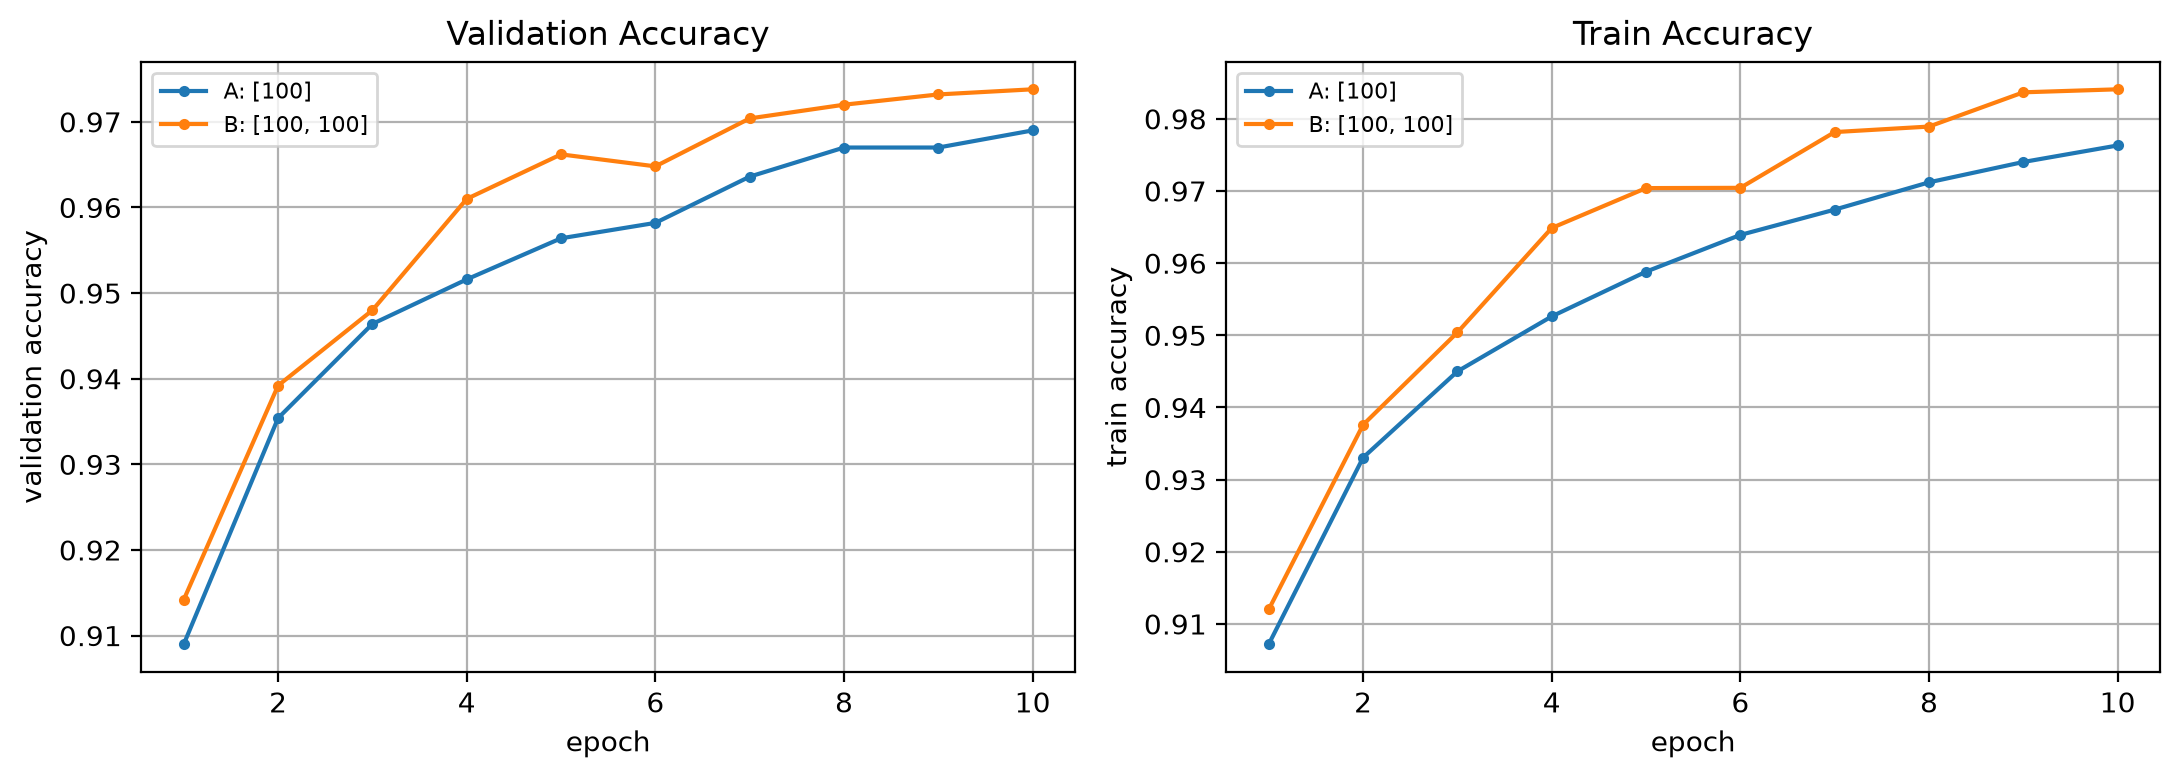
\includegraphics[width=0.88\linewidth]{mlp_compare.png}
\figcap{왼쪽: epoch마다의 검증 정확도, 오른쪽: 훈련 정확도}
\raggedright
\begin{itemize}
\item 두 신경망 모두 10 epoch까지 정확도가 \textbf{아직 오르고 있다} $\to$ epoch를 늘려 볼 만하다
\item 훈련 정확도와 검증 정확도의 차이: A는 $0.73\%$p, B는 $1.03\%$p. 신경망이 클수록 차이가 커지는지 지켜보자 (과적합)
\end{itemize}
\end{frame}

% =================================================
\section{최종 평가: test는 한 번만}
% =================================================

\begin{frame}[fragile]{6. 검증 정확도로 고르고, test는 한 번}
\begin{lstlisting}
best_name = max(results, key=lambda k: results[k][1]["val_acc"][-1])
best_net = results[best_name][0]
test_acc = best_net.accuracy(x_test, t_test)
print(f"\nbest on validation: {best_name}")
print(f"test accuracy of the chosen network: {test_acc:.4f}")
\end{lstlisting}
\begin{lstlisting}[style=outstyle]
best on validation: B: [100, 100]
test accuracy of the chosen network: 0.9733
\end{lstlisting}
\begin{itemize}
\item \code{max(results, key=...)}: 딕셔너리의 키(이름) 중에서 \code{key} 함수의 값이 가장 큰 것
\begin{itemize}
\item \code{results[k][1]}: 기록 \code{hist}, \code{["val\_acc"][-1]}: 마지막 epoch의 검증 정확도
\end{itemize}
\item test 정확도는 \textbf{고른 신경망 하나에 대해서만} 계산한다: $97.33\%$
\item 검증 정확도 $97.38\%$와 비슷하다 $\to$ 검증 데이터로 고른 것이 처음 보는 데이터에도 통했다
\end{itemize}
\end{frame}

\begin{frame}[fragile]{6. 혼동행렬 만들기}
\begin{lstlisting}
pred = np.argmax(best_net.predict(x_test), axis=1)
C = np.zeros((10, 10), dtype=int)
for t, p in zip(t_test_o, pred):
    C[t, p] += 1
...
print("per-class test accuracy:", np.round(np.diag(C) / C.sum(axis=1), 4))
\end{lstlisting}
\begin{lstlisting}[style=outstyle]
per-class test accuracy: [0.9786 0.9903 0.9729 0.9693 0.9827 0.9809 0.9749 0.9475 0.9795 0.9564]
\end{lstlisting}
\begin{itemize}
\item \textbf{혼동행렬} $C$: $C_{ij}=$ ``정답이 $i$인데 $j$로 예측한 test 이미지의 수''
\item \code{zip(t\_test\_o, pred)}: (정답, 예측)의 쌍을 하나씩. 여기서는 one-hot이 아닌 \textbf{원래 번호}를 쓴다
\item 대각선 \code{np.diag(C)}: 맞힌 수. 행의 합 \code{C.sum(axis=1)}: 그 숫자의 test 이미지 수
\item 클래스별 정확도가 가장 낮은 숫자: \textbf{7} ($94.75\%$), 그다음 \textbf{9} ($95.64\%$)
\end{itemize}
\end{frame}

\begin{frame}{6. 혼동행렬: \code{mlp\_confusion.png}}
\begin{columns}[c,onlytextwidth]
\begin{column}{0.52\textwidth}
\centering
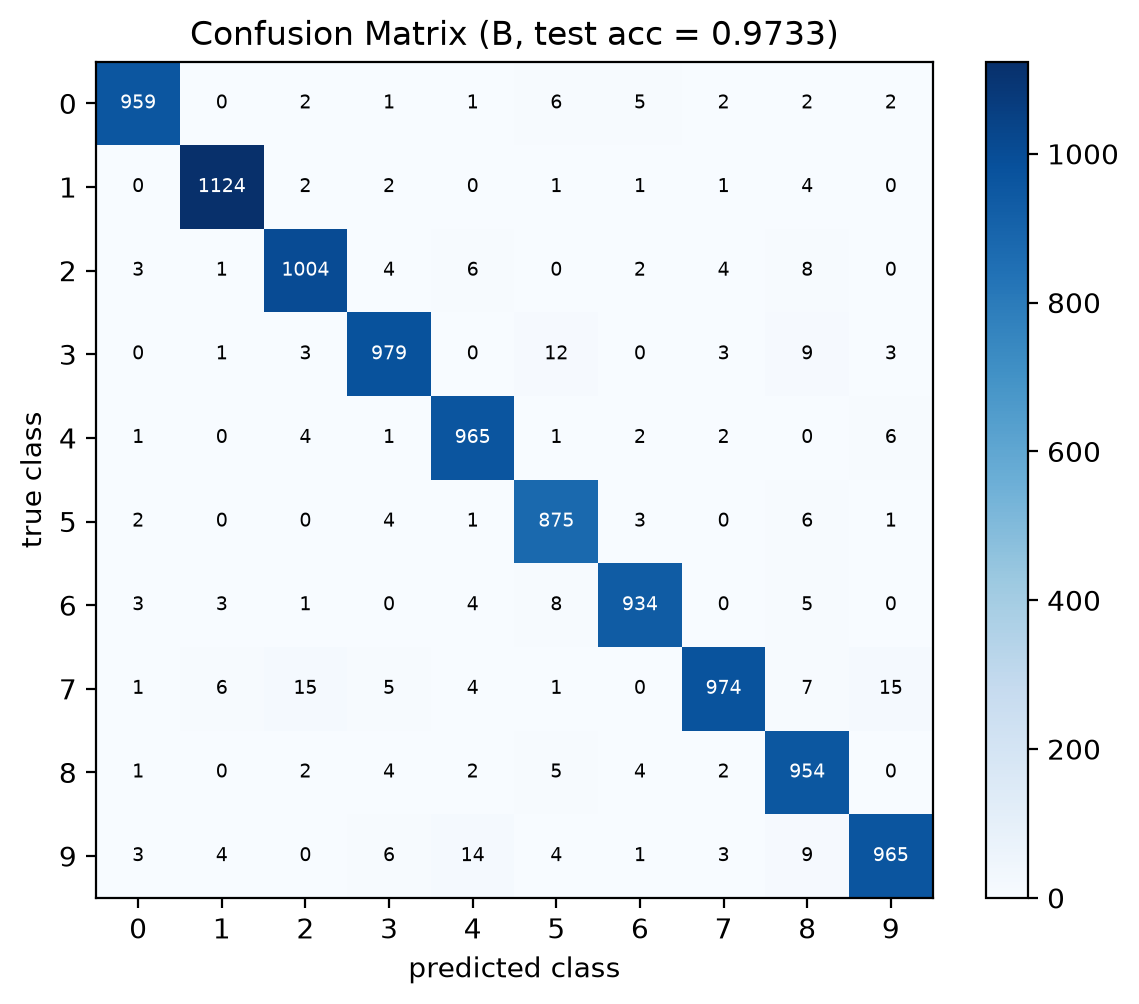
\includegraphics[height=0.78\textheight]{mlp_confusion.png}
\end{column}
\begin{column}{0.44\textwidth}
\small
\begin{itemize}
\item 대각선이 진하다: 대부분 맞힌다
\item 대각선 밖에서 큰 칸 (정답 $\to$ 예측):
\begin{itemize}
\item $7\to2$: 15장, \ $7\to9$: 15장
\item $9\to4$: 14장
\item $3\to5$: 12장
\end{itemize}
\item 모양이 비슷한 숫자끼리 헷갈린다
\item 혼동행렬은 대칭이 아니다: $7\to2$는 15장이지만 $2\to7$은 4장
\end{itemize}
\vskip2mm
\begin{thinkbox}
\small 틀린 이미지를 직접 그려 보면 사람도 헷갈릴 만한 것이 많을까?
\end{thinkbox}
\end{column}
\end{columns}
\end{frame}

% =================================================
\section{정리와 과제 2}
% =================================================

\begin{frame}{정리}
\begin{keybox}[이번 시간의 핵심]
\footnotesize
\begin{itemize}\setlength{\itemsep}{0.6mm}
\item \textbf{데이터}: \code{reshape(N, -1)}로 펼치고 \code{/255}로 정규화, \code{np.eye(10)[t]}로 one-hot. 훈련 55000 / 검증 5000 / test 10000
\item \textbf{계층}: \code{forward}는 값을 저장하고 \code{backward}는 저장한 값으로 입력의 기울기를 돌려준다. 기울기의 shape $=$ 변수의 shape
\item \textbf{출력층}: softmax는 최댓값을 빼고 계산. cross entropy와 함께 쓰면 역전파의 출발이 $\frac1h(Y-T)$
\item \textbf{\code{MultiLayerNet}}: \code{sizes} 목록으로 Affine--활성화를 리스트에 쌓는다. 순전파는 앞에서부터, 역전파는 \code{reversed}
\item \textbf{학습}: epoch마다 섞고 100개씩. 갱신은 \code{-=} (계층과 같은 배열을 제자리에서)
\item \textbf{평가}: 설정은 \textbf{검증 정확도}로 고르고, test는 고른 신경망에 \textbf{한 번만}. 혼동행렬로 어디서 틀리는지 본다
\item 결과: \code{[100, 100]}이 검증 $97.38\%$로 선택, test $97.33\%$
\end{itemize}
\end{keybox}
\end{frame}

\begin{frame}{과제 2: MNIST 정확도 98\% 도전}
\small
\code{experiments} 리스트에 한 줄씩 추가하며 실험하자. 한 번에 \textbf{한 가지만} 바꾼다.
\vskip1mm
\centering
\footnotesize
\renewcommand{\arraystretch}{1.15}
\begin{tabular}{lll}
\toprule
\textbf{바꿀 것} & \textbf{어디를} & \textbf{예} \\
\midrule
깊이 (은닉층 수) & 둘째 항목 & \code{[100, 100, 100]} \\
넓이 (node 수) & 둘째 항목 & \code{[300]}, \code{[256, 128]} \\
활성화 함수 & 셋째 항목 & \code{"sigmoid"} \\
손실 함수 & 넷째 항목 & \code{"se"} (제곱 오차) \\
학습률 & 다섯째 항목 & \code{0.05}, \code{0.2} \\
미니배치 크기 & 여섯째 항목 & \code{50}, \code{200} \\
epoch 수 & \code{epochs = 10} & \code{20}, \code{30} \\
\bottomrule
\end{tabular}
\raggedright
\small
\begin{itemize}
\item 시도한 설정과 결과(train/검증 정확도, 그래프)를 \textbf{표로} 정리하고, test 정확도는 \textbf{최종 선택한 신경망만} 보고
\item 어떤 요인의 영향이 가장 컸는지, 과적합의 징후(train과 검증의 차이)가 있었는지 설명
\end{itemize}
\end{frame}

\begin{frame}{실습 문제}
\small
\begin{enumerate}
\item \code{MultiLayerNet(784, [256, 128], 10)}의 매개변수 수를 손으로 계산하고 \code{num\_params()}로 확인하기
\item \code{train}이 epoch마다 \textbf{평균 손실}을 출력하도록 고치기 (힌트: \code{hist["loss"]}의 마지막 \code{iter\_per\_epoch}개)
\item 갱신 줄을 \code{network.params[key] = network.params[key] - learning\_rate * grads[key]}로 바꾸면 정확도가 어떻게 되는가? 이유는?
\item 은닉층 넓이는 그대로 두고 깊이만 $1, 2, 3, 4$로 늘려 검증 정확도와 실행 시간을 비교하기
\item 매개변수 수가 비슷한 \textbf{넓은} 신경망(\code{[113]} 정도)과 \textbf{깊은} 신경망(\code{[100, 100]})을 비교하기
\item 혼동행렬에서 $7\to2$로 틀린 test 이미지를 찾아 그리기 (힌트: \code{np.where((t\_test\_o == 7) \& (pred == 2))})
\item \code{weight\_init\_std}를 $0.5$와 $0.001$로 바꾸고 \code{[100, 100, 100, 100]}을 학습시키면? (가중치 초기화가 왜 중요한가)
\end{enumerate}
\end{frame}

\end{document}
